\subsection{Positioning elements}

Layout is always an important factor when using a visual language:
A well laid-out diagram is easiest to understand and, by centralizing important
elements or clustering related elements, you can actually impart additional information.

\begin{enumerate}
\item[$\blacktriangleright$] To select a group of elements, either drag a selection box around the items or hold \texttt{Ctrl} and select each element
one-by-one.

\item[$\blacktriangleright$] In the top right corner of the last selected element, a small colon-styled symbol will appear (\Cref{ea:layout1}). Click on
this for a context list of different options you can simultaneously apply to all active elements. The same list appears on the toolbar above the
diagram. 

\item[$\blacktriangleright$] Experiment to find out what effect each option has. The last symbol in the list opens a further drop-down menu with standard layout
algorithms to organize your diagram automatically.

\item[$\blacktriangleright$] Right-clicking any of the selected elements opens a different menu with a further set of layout options and their descriptions
(\Cref{ea:layout2}). \texttt{Align Centers} or \texttt{Same Height and Width} can be especially useful.

\begin{figure}[htbp]
\begin{center} 
  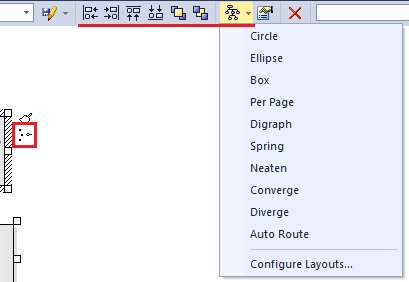
\includegraphics[width=0.65\textwidth]{ea_layoutElementsCommonContext}
  \caption{Setting the layout of multiple elements}  
  \label{ea:layout1}
\end{center}
\end{figure}

\begin{figure}[htbp]
\begin{center}  
  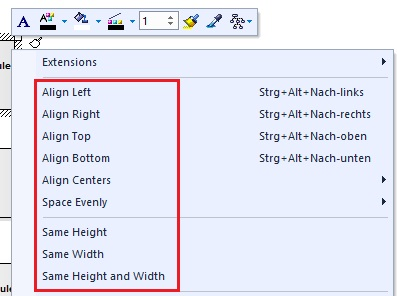
\includegraphics[width=0.7\textwidth]{layoutElements2}
  \caption{Further layout options}  
  \label{ea:layout2} 
\end{center}
\end{figure}

\end{enumerate}
